% !TEX root = RKWard_paper.tex
\section{Extending RKWard - an example of creating a plugin}
\label{sec:example_plugin}
As discussed in Section~\ref{sec:technical_plugins}, plugins in RKWard are
defined by four separate files (Figure~\ref{fig:plugin_structure}). To give an impression of the technique,
this section shows (portions of) the relevant files for a plugin that provides
a simple dialog for a t-test. For brevity, the help-file is omitted.

\subsection{Defining the menu hierarchy}
\label{sec:defining_menu_hierarchy}
A so called ``.pluginmap'' file declares each plugin, and, if appropriate, defines where it should
be placed in the menu hierarchy. Usually each .pluginmap-file declares many plugins. In this example
we only show one, namely, the definition entry for a two variable t-test (see Figure~\ref{fig:ttest-gui-example}). 
The pluginmap (\code{<!DOCTYPE rkpluginmap>}) gives a unique identifier (``id"), the location of the GUI description (``file"), and the window title (``label''). The menu
is defined in a hierarchical structure (see code example below\footnote{Long lines are broken at ``$\ldots~\ldots$''.}). Moreover, the position within the menu can be explicitly defined.
This might be required if the menu entries are to be ordered non-alphabetically.

\begin{footnotesize}
\begin{Code}
<!DOCTYPE rkpluginmap>

<document base_prefix="" namespace="rkward">
  <components>
    <component type="standard" id="t_test_two_vars" file="analysis/t_test_two_vars.xml" ...
      ... label="Two Variable t-test" />
  </components>

  <hierarchy>
    <!-- Menu hierarchy can be defined in XML, easily.
    Menus with the same "id"-attribute will be merged, even if defined in
    separate .pluginmap files. -->
    <menu id="analysis" label="Analysis" index="4">
      <menu id="means" label="Means" index="4">
        <menu id="ttests" label="t-Tests">
          <entry component="t_test_two_vars" />
        </menu>
      </menu>
    </menu>
  </hierarchy>
</document>
\end{Code}
\end{footnotesize}


\begin{figure}[htp]
 \centering
 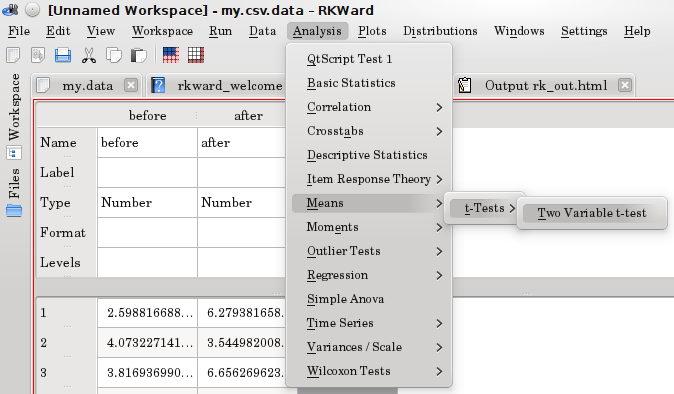
\includegraphics{../figures/ttest-gui-example.png}
 \caption{Generated menu GUI as defined by the plugin map.}
 \label{fig:ttest-gui-example}
\end{figure}


\subsection {Defining the dialog UI}
\label{sec:defining_dialog_ui}
The main \proglang{XML} file of each plugin defines the layout and behavior of the GUI, and references the
\proglang{ECMAScript} file that is used for generating \proglang{R} code from UI settings and the help file (not included in this paper).

Some GUI behavior can also be scripted in \proglang{ECMAScript}. In this example, the logic is defined in \proglang{XML} (the ``Assume equal variances'' checkbox
is only enabled for paired sample tests).

The \proglang{XML} file defines the t-test plugin (\code{<!DOCTYPE rkplugin>}) to be organized in two tabs (Figure~\ref{fig:t_test}A) asking for the variables
to analyze in the first tab and optionally in the second tab for specific settings like the confidence level (default 0.95). Note that this \proglang{XML} file
also invokes the \proglang{XML} help file. Two variables can be selected (\code{<varslot .../>}). These are set to be ``required'', i.\,e.
the ``Submit'' button will remain disabled until the user has made a valid selection for both.

\begin{footnotesize}
\begin{Code}
<!DOCTYPE rkplugin>
<document>
  <code file="t_test_two_vars.js"/>
  <help file="t_test_two_vars.rkh"/>

  <logic>
    <!-- GUI behavior can also be scripted in ECMAScript. -->
    <connect client="varequal.enabled" governor="paired.not"/>
  </logic>

  <dialog label="Two Variable t-Test">
    <tabbook>
      <tab label="Basic settings" id="tab_variables">
        <row id="basic_settings_row">
          <varselector id="vars"/>
          <column>
            <varslot type="numeric" id="x" source="vars" required="true"
              label="compare"/>                                                             
            <varslot type="numeric" id="y" source="vars" required="true"
              label="against"/>
            <radio id="hypothesis" label="using test hypothesis">
              <option value="two.sided" label="Two-sided"/>
              <option value="greater" label="First is greater"/>
              <option value="less" label="Second is greater"/>
            </radio>
            <checkbox id="paired" label="Paired sample" value="1" value_unchecked="0" />
          </column>
        </row>
      </tab>
      <tab label="Options" id="tab_options">
        <checkbox id="varequal" label="assume equal variances" value="1"
          value_unchecked="0"/>
        <frame label="Confidence Interval" id="confint_frame">
          <spinbox type="real" id="conflevel" label="confidence level" min="0" max="1"
            initial="0.95"/>
          <checkbox id="confint" label="print confidence interval" value="1"
            checked="true"/>
        </frame>
        <stretch/>
      </tab>
    </tabbook>
  </dialog>
</document>
\end{Code}
\end{footnotesize}

\subsection{Generating R code from UI settings}
\label{sec:generating_r_code_from_ui_settings}
A simple \proglang{ECMAScript} script is used to generate \proglang{R} code from UI settings (using \code{echo()} commands).
Generated code for each plugin is divded into three sections: ``Preprocess'', ``Calculate'', and ``Printout'', although each
may be empty.

\begin{footnotesize}
\begin{Code}
// globals
var x;
var y;
var varequal;
var paired;

function preprocess () {
  x = getValue ("x");
  y = getValue ("y");

  echo ('names <- rk.get.description (' + x + ", " + y + ')\n');
}

function calculate () {
  varequal = getValue ("varequal");
  paired = getValue ("paired");

  var conflevel = getValue ("conflevel");
  var hypothesis = getValue ("hypothesis");

  var options = ", alternative=\"" + hypothesis + "\"";
  if (paired) options += ", paired=TRUE";
  if ((!paired) && varequal) options += ", var.equal=TRUE";
  if (conflevel != "0.95") options += ", conf.level=" + conflevel;

  echo ('result <- t.test (' + x + ", " + y + options + ')\n');
}

function printout () {
  echo ('rk.header (result\$method, \n');
  echo ('  parameters=list ("Comparing", paste (names[1], "against", names[2]),\n');
  echo ('  "H1", rk.describe.alternative (result)');
  if (!paired) {
    echo (',\n');
    echo ('  "Equal variances", "');
    if (!varequal) echo ("not");
    echo (' assumed"');
  }
  echo ('))\n');
  echo ('\n');
  echo ('rk.results (list (\n');
  echo ('  \'Variable Name\'=names,\n');
  echo ('  \'estimated mean\'=result\$estimate,\n');
  echo ('  \'degrees of freedom\'=result\$parameter,\n');
  echo ('  t=result\$statistic,\n');
  echo ('  p=result\$p.value');
  if (getValue ("confint")) {
    echo (',\n');
    echo ('  \'confidence interval percent\'=(100 * attr(result\$conf.int, "conf.level")),\n');
    echo ('  \'confidence interval of difference\'=result\$conf.int ');
  }
  echo ('))\n');
}
\end{Code}
\end{footnotesize}

The generated code readable by the user is the following \proglang{R} code (code below and Figure~\ref{fig:t_test}). 
Here, \code{rk.header} and \code{rk.results} 
are RKWard functions provided by the package \pkg{rkward}. In case the package is installed the code below 
can be run from any \proglang{R} engine.

\begin{footnotesize}
\begin{Code}
local({
## Prepare
names <- rk.get.description (my.csv.data[["before"]], my.csv.data[["after"]])
## Compute
result <- t.test (my.csv.data[["before"]], my.csv.data[["after"]], alternative="less", paired=TRUE)
## Print result
rk.header (result$method, 
	parameters=list ("Comparing", paste (names[1], "against", names[2]),
	"H1", rk.describe.alternative (result)))

rk.results (list (
	'Variable Name'=names,
	'estimated mean'=result$estimate,
	'degrees of freedom'=result$parameter,
	t=result$statistic,
	p=result$p.value,
	'confidence interval percent'=(100 * attr(result$conf.int, "conf.level")),
	'confidence interval of difference'=result$conf.int ))
})

\end{Code}
\end{footnotesize}